
\section{Experiments}
\label{sec:experiments}

In this section, we wish to experimentally evaluate two criteria: the
performance of the different optimisation algorithms to minimise the \addkrrs
objective \eqref{eqn:optObjective}, and the performance of \addkrrs and other
nonparametric regression methods. So far, we only have results on synthetic
data.


\begin{figure*}
\centering
\subfigure[]{
  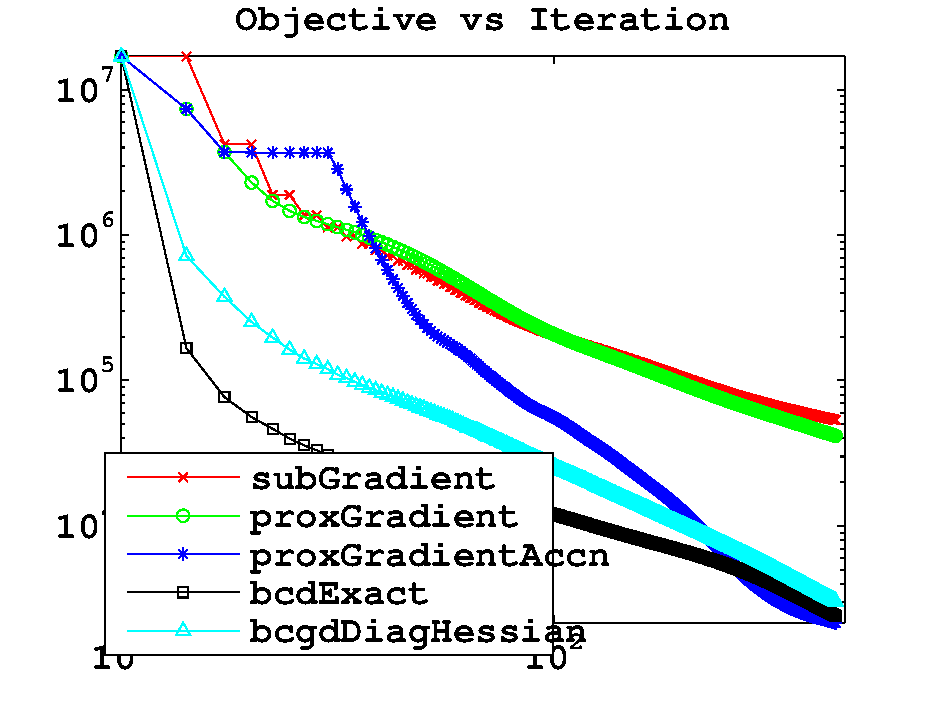
\includegraphics[width=\imarrwthree]{figs/iteration2000v1} \hspace{\imhspthree}
  \vspace{\imlabelspace}
  \label{fig:iteration}
}
\subfigure[]{
  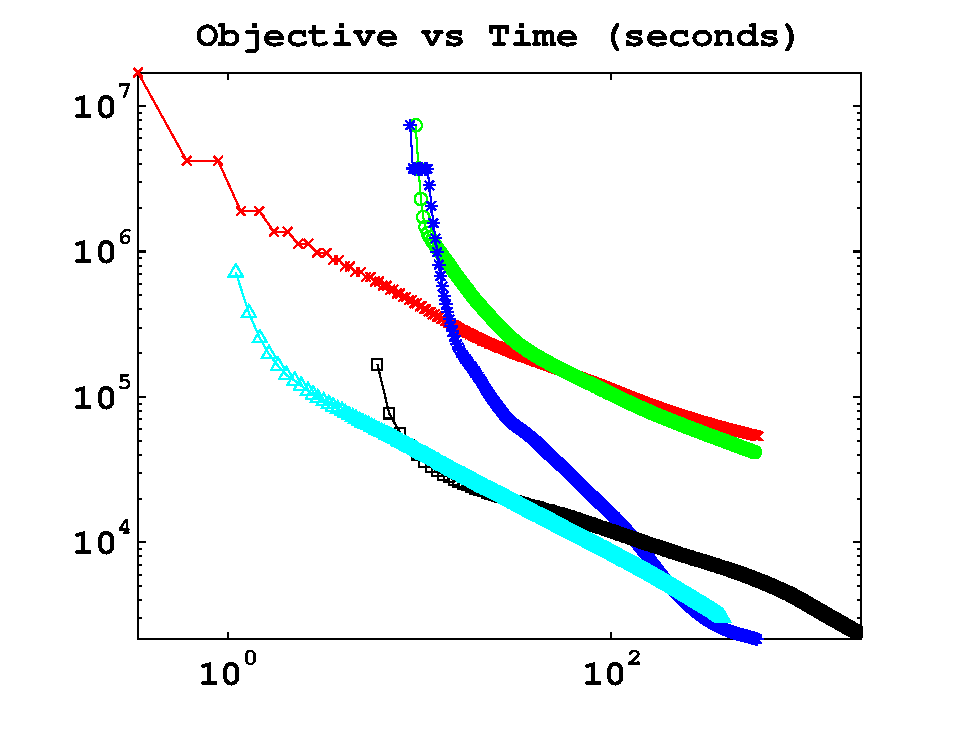
\includegraphics[width=\imarrwthree]{figs/time2000v1} \hspace{\imhspthree}
  \vspace{\imlabelspace}
  \label{fig:time}
}
\subfigure[]{
  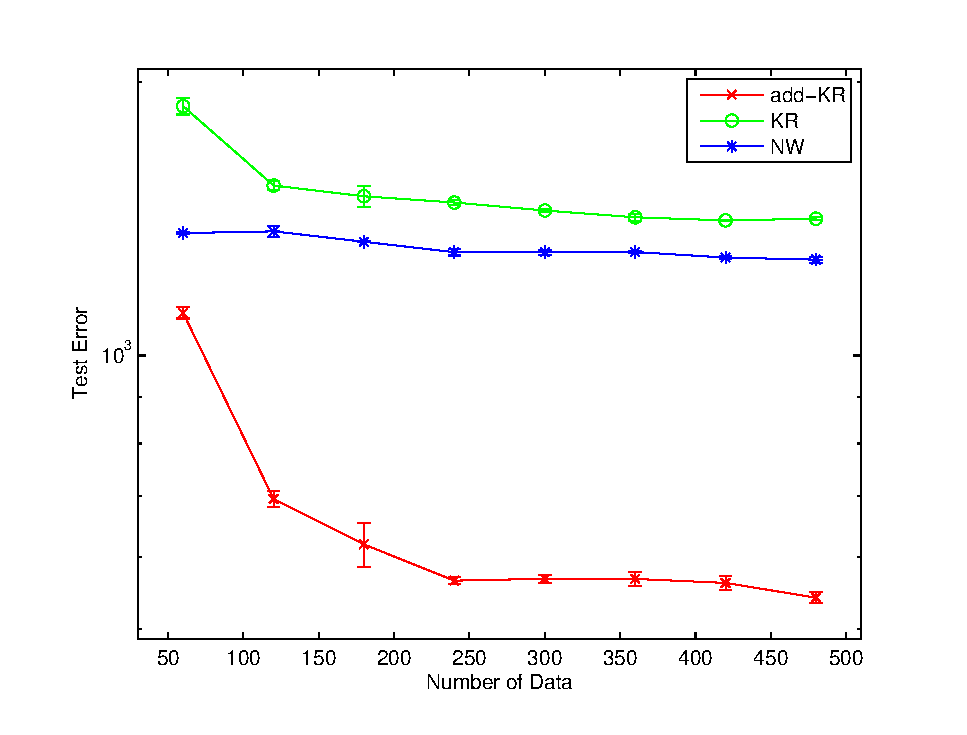
\includegraphics[width=\imarrwthree]{figs/toyResults}
  \vspace{\imlabelspace}
  \label{fig:compare}
} \\
\caption[]{ \hspace{-0.1in}
Figures~\subref{fig:iteration} and~\subref{fig:time} plot the objective value vs
iteration and cpu time respectively. Accelerated proximal gradient descent (blue
curve) seems to perform best. Figure~\subref{fig:compare} plots the test set
error for \addkrrs, \krrs and \nws on a synthetic problem. 
\addkrrs outperforms both methods.
}
\label{fig:toythree}
\vspace{\imtextspace}
\end{figure*}

